\documentclass[12pt,titlepage,a4page , tikz , multi,table , svgnames,xcdraw]{article}
\usepackage{graphicx}
\usepackage[svgnames , table , xcdraw]{xcolor} 
\usepackage{fancyhdr}
 
\usepackage{hyperref}
\hypersetup{
    colorlinks=true,
    linkcolor=blue,
    filecolor=magenta,      
    urlcolor=cyan,
}
\usepackage{multirow}
\usepackage{graphicx}
\usepackage{float}
\usepackage{enumitem}
\usepackage{listings }
\usepackage[a4paper, total={6in, 8in}]{geometry}
\usepackage{afterpage}
\usepackage{amssymb}
\usepackage{lscape}
\usepackage{amsmath}
\usepackage{svg}
\usepackage[final]{pdfpages}



\usepackage[T1]{fontenc}
\usepackage{tikz}
\usepackage[utf8]{inputenc} % Required for inputting international characters
\usepackage{PTSerif} 

\usepackage{float}

\usepackage{xepersian}
\settextfont[
 BoldFont={XB NiloofarBd.ttf}
 ]{XB Niloofar.ttf}


\NewDocumentCommand{\codeword}{v}{
\texttt{\textcolor{blue}{#1}}
}
\DeclareFixedFont{\ttb}{T1}{txtt}{bx}{n}{12} % for bold
\DeclareFixedFont{\ttm}{T1}{txtt}{m}{n}{12}  % for normal


\definecolor{deepblue}{rgb}{0,0,0.5}
\definecolor{deepred}{rgb}{0.6,0,0}
\definecolor{deepgreen}{rgb}{0,0.5,0}


% Python style for highlighting
\newcommand\pythonstyle{\lstset{
language=Python,
basicstyle=\ttm,
otherkeywords={self},             % Add keywords here
keywordstyle=\ttb\color{deepblue},
emph={MyClass,__init__},          % Custom highlighting
emphstyle=\ttb\color{deepred},    % Custom highlighting style
stringstyle=\color{deepgreen},
frame=tb,                         % Any extra options here
showstringspaces=false            % 
}}


% Python environment
\lstnewenvironment{python}[1][]
{
\pythonstyle
\lstset{#1}
}
{}

% Python for external files
\newcommand\pythonexternal[2][]{{
\pythonstyle
\lstinputlisting[#1]{#2}}}

% Python for inline
\newcommand\pythoninline[1]{{\pythonstyle\lstinline!#1!}}


\begin{document}

\begin{titlepage}

 \begin{center}
        
       \vspace*{1cm}

 \vspace{1cm}
       \textbf{ \Huge{به نام خدا} }
       \vspace{0.4cm}
       
       
\includegraphics[width=0.4\textwidth]{sharif1.png}
       
 	\vspace{0.7cm}
       \textbf{ \LARGE{هوش مصنوعی} }

 
   \vspace{0.7cm}
  \textbf{ \Large{ تمرین پیاده‌سازی سوم} }
   \vspace{0.5cm}
       
 
      \large \textbf{دانشکده مهندسی کامپیوتر}\\\vspace{0.2cm}
    \large   دانشگاه صنعتی شریف\\\vspace{0.25cm}
      
استاد:\\
    \textbf{{جناب آقای دکتر عبدی}}

    \vspace{0.25cm}
    \noindent\rule[1ex]{\linewidth}{3pt}
    
    \vspace{0.5cm}
نام و نام خانوادگی:\\
    \textbf{{امیرمهدی نامجو}}
        \vspace{0.1cm}

\end{center}
\end{titlepage}

\newpage
\pagestyle{fancy}
\fancyhf{}
\fancyfoot{}

\cfoot{\thepage}
\chead{تمرین پیاده‌سازی سوم}
\rhead{امیرمهدی نامجو}
\lhead{هوش مصنوعی}



\newpage



\section{کتابخانه‌های موردنیاز}

ابتدا باید این پکیج‌ها برای اجرای درست کد نصب شوند. دستور نصب هر کدام در زیر آمده است:

\begin{latin}
\begin{lstlisting}[language=Python]
pip install numpy
pip install sklearn
pip install tensorflow
pip install matplotlib
\end{lstlisting}

\end{latin}
از sklearn برای پیاده‌سازی خود \lr{SVM،} از tensorflow و به طور دقیق‌تر Keras برای لود کردن دیتاست بخش دوم و از matplotlib برای رسم نمودار استفاده شده است. با این وجود در فایل requirements هم بخش اصلی کتابخانه‌های موجود رو کامپیوتر من قرار دارد تا در صورت وجود مشکل، با نصب همه آن‌ها مشکل برطرف شود.

ضمناً همه کدها بر روی \lr{Python 3.8} تست شده است و تضمینی برای اجرای درست آن‌ها بر روی نسخه‌های قدیمی‌تر (مخصوصاً به دلیل تغییراتی که بعضاً در سینتکس کدها در نسخه‌های مخلتف پایتون داده می‌شود) وجود ندارد. البته احتمالاً در همه نسخه‌های \lr{3.0} به بالای پایتون که کتابخانه‌های بالا امکان نصب داشته باشند، کدها به درستی اجرا خواهند شد ولی به هر حال در صورت اجرای نادرست، باید پایتون 64 بیتی نسخه \lr{3.8} را نصب کرد.




\newpage

\section{بخش اول}

\subsection{توضیحات کد}
در ابتدا بخش‌های مختلف کد را توضیح می‌دهم:


\begin{latin}
\begin{python}[language=Python]
def plot_svc(model):
    """Plot the decision function for a 2D SVC"""
    ax = plt.gca()
    xlim = ax.get_xlim()
    ylim = ax.get_ylim()

    # create grid to evaluate model
    x = np.linspace(xlim[0], xlim[1], 30)
    y = np.linspace(ylim[0], ylim[1], 30)
    Y, X = np.meshgrid(y, x)
    xy = np.vstack([X.ravel(), Y.ravel()]).T
    P = model.decision_function(xy).reshape(X.shape)

    # plot decision boundary and margins
    ax.contour(X, Y, P, colors='k',
               levels=[-1, 0, 1], alpha=0.5,
               linestyles=['--', '-', '--'])

    # plot support vectors
    ax.scatter(model.support_vectors_[:, 0],
               model.support_vectors_[:, 1],
               s=300, linewidth=1, facecolors='none');
    ax.set_xlim(xlim)
    ax.set_ylim(ylim)
\end{python}

\end{latin}

این تابع یک فایل مدل که در اصل نتیجه Train شده SVM به کمک sklearn است، را به عنوان ورودی گرفته و سپس با کمک اطلاعات ذخیره شده در آن، هم نقاط را رسم کرده و هم این که با کمک متغیر \lr{support\_vectors\_} و همچنین سایر اطلاعات ذخیره شده در مدل، در بخش اول به کمک تابع contour خطوط مارجین و به کمک بخش دوم خود خط جداکننده اصلی را به درستی رسم می‌کند.

تابع بعدی:


\begin{latin}
\begin{python}[language=Python]
def kfold_svm(X, y, number_of_folds=5, kernel='rbf', C=1,
 gamma='auto', degree=5, coef0=0.0):
    clf = svm.SVC(kernel=kernel, C=C, gamma=gamma,
     degree=degree, coef0=coef0)
    cross_validate_result = cross_validate(clf, X, y, 
    cv=number_of_folds, scoring='accuracy',
     return_estimator=True, return_train_score=True)
     
    clfs = cross_validate_result['estimator']
    train_scores = cross_validate_result['train_score']

	test_scores = cross_validate_result['test_score']

    print("train_scores: " )
    print(train_scores)
    print()
    print("test_scores: " )
    print(test_scores)
    best_one_index = np.argmax(test_scores)

    return clfs[best_one_index], test_scores[best_one_index]
\end{python}

\end{latin}

است. این تابع در اصل قلب اصلی کد است. با کمک ورودی‌هایی که به آن داده می‌شود، یک مدل \lr{Suppor Vector Classifier} با موارد تعیین شده ساخته شده، سپس از طریق مقدار \lr{number\_of\_folds} روش \lr{Cross Validation} به صورت $n-fold$ انجام می‌گیرد (یعنی داده‌ها مثلاً به 5 قسمت تقسیم می‌شوند و در 5 بار متوالی، یک بار قسمت اول تست و بقیه داده‌اموزشی، بار بعدی قسمت دوم تست و بقیه قسمت آموزشی و... خواهند بود) و نتایج همه حالات ذخیره می‌شود. در نهایت نتایج Fold های هم برای  تست و هم آموزش چاپ شده و بهترین مدل به همراه نمره آن که بر اساس دقت تقسیم بندی درست (یعنی درصد داده‌هایی که درست تقسیم‌شده‌اند) داده‌های تست به دست آمده است،  به عنوان خروجی داده می‌شود. 

بخش بعدی کد، یک تابع است که به ازای تست کیسه‌ای مختلف تابع را اجرا می‌کند. از آن جایی که کد آن صرفاً از یکسری بخش تکراری تشکیل شده، به جای کد حالت‌های مختلف آن را شرح می‌دهم که با ورودی دادن عددهای مختلف به عنوان آی دی تست کیس اجرا می‌شوند و در هنگام اجرای برنامه به طور کامل نوشته می‌شوند.

حالت 0: دو دابره تو در تو با کرنل RBF و گاما \lr{1}

حالت 1: دو دابره تو در تو با کرنل چندجمله‌ای درجه \lr{5} و ضریب ثابت \lr{0.5}

حالت 2: دو دابره تو در تو با کرنل خطی که نتیجه خوبی به دست نمی‌دهد.

حالت 10: دو دایره تو در تو و نزدیک‌تر متفاوت با کرنل RBF و گاما \lr{1}

حالت 11: دو دایره تودرتو  و نزدیک‌تر با کرنل RBF و گاما \lr{1000} در این حالت Overfit رخ می‌دهد.

حالت 12: دو دابره تو در تو و نزدیک‌تر با کرنل چند خطی که نتیجه خوبی به دست نمی‌دهد.

حالت 13: دو دابره تو در تو و نزدیک‌تر با کرنل چندجمله‌ای درجه \lr{5} و ضریب ثابت \lr{0.5}

حالت 20: دو هلال با کرنل RBF و گاما \lr{1}

حالت 21: دو هلال با کرنل RBF و گاما \lr{1000} که Overfit شدید رخ می‌دهد

حالت 22: دو هلال با کرنل چندجمله‌ای درجه \lr{3} و ضریب ثابت \lr{0.5}

حالت 23: دو هلال با کرنل خطی

حالت 24: دو هلال با کرنل rbf و گاما \lr{1} و \lr{C=0.0001} در اصل C در بقیه موارد همیشه $1$ بوده و هر چه مقدار آن کمتر باشد، یعنی حساسیست و توجه الگوریتم نسبت به داده‌ها به نوعی کمتر می‌شود. در اصل $C$ را ضریب عادی سازی می‌دانند و زیاد بودن آن معمولاً باعث Overfit بیش از اندازه شده و کم بودن بیش از اندازه‌اش هم می‌تواند باعث نتایج نادرست بشود.

حالت 30: دو تکه جدا از هم با کرنل RBF و گاما \lr{1}


حالت 31: دو تکه جدا از هم با کرنل چندجمله‌ای درجه \lr{3} و ضریب ثابت \lr{0.5}

حالت 32: دو تکه جدا از هم با کرنل خطی

حالت 40: دو تکه جدا از هم اما نزدیک‌تر با کرنل RBF و گاما \lr{1}. در این حالت اندکی Overfit پیش آمده ولی نه خیلی زیاد


حالت 41: دو تکه جدا از هم اما نزدیک‌تر  با کرنل چندجمله‌ای درجه \lr{3} و ضریب ثابت \lr{0.5}

حالت 42: دو تکه جدا از هم اما نزدیک‌تر با کرنل خطی


در نهایت بعد از این موارد، بخش مربوط به نوشتن حالات مختلف و درخواست ورودی از کاربر و اجرای کد و رسم شکل قرار گرفته است.

\subsection{نتایج}

در تست هایی که من روی حالت‌های مختلف انجام دادم، تقریباً در اکثر اوقات کرنل RBF عملکرد خوبی از خودش نشان می‌داد. در مواردی نظیر دو تکه جدا از هم که واقعاً قسمت‌ها جدا بودند، کرنل خطی هم عملکرد خوبی داشت ولی مثلاً برای دایره، عملکرد کرنل خطی بسیار بد است و تقریباً دقت 50 درصدی یعنی کاملاً تصادفی را به دست می‌آورد. از سوی دیگر در مورد کرنل‌های چندجمله‌ای هم معمولاً در حالت‌هایی نظیر دایره‌ها، با درجات 5 به بالا و البته همراه با یک ضریب ثابت ناصفر به نتیجه مطلوب می‌رسیم. در حالت دو هلال هم شکل کلی آن‌ها تقریباً شبیه چندجمله‌ای درجه 3 است و همین چندجمله‌ای می‌تواند به خوبی جواب گو باشد.

چند نتیجه مهمی که گرفته شد، یکی در مورد ضریب گاما در کرنل rbf بود. کرنل rbf به شکل زیر تعریف می‌شود:

$$K\left(\mathbf{x}, \mathbf{x}^{\prime}\right)=\exp \left(-\frac{\left\|\mathbf{x}-\mathbf{x}^{\prime}\right\|^{2}}{2 \sigma^{2}}\right)$$

و یا به فرم دیگر:

$$K\left(\mathbf{x}, \mathbf{x}^{\prime}\right)=\exp \left(-\gamma\left\|\mathbf{x}-\mathbf{x}^{\prime}\right\|^{2}\right)$$

و در اصل کرنلی است که داده‌ها را به یک فضای بی‌نهایت بعدی نگاشت می‌دهد. گاما خیلی زیاد، باعث می‌شود که مدل دچار Overfitting شدید بشود، زیرا باعث می‌شود که ناحیه تأثیر خط اصلی جدا کننده، صرفاً خود آن در نظر گرفته بشود و در نتیجه، خط جدا کننده طوری ایجاد می‌شود که دقیقاً داده‌ها را جدا سازی کند. از سوی دیگر گاما خیلی کم هم باعث می‌شود که اصلاً ساختار کلی داده‌ها درک نشوند و تقریباً سیستم شبیه یک جداکننده خطی عمل کند. در نتیجه انتخاب گاما مناسب اهمیت بالایی دارد و در تست کیس ها هم من سعی کردم هم اثر گاما زیاد و هم اثر گاما کم را در مواردی آزمایش کرده باشم.

در صفحات بعد، شکل‌های تمامی حالات شهر داده شده در بالا به همان ترتیب آورده شده است.


به دلیل زیاد بودن تست کیس ها، نتایج دقت‌های آن‌ها به صورت موردی آورده نشده است. با این حال، شکل‌ها تا حد خوبی گویا هستند و خود نتایج عددی هم به راحتی با اجرای کد نمایش داده می‌شوند.


ضمناً تولید تست کیس ها از طریق توابع آماده \lr{make\_blobs} و \lr{make\_circles} و \lr{make\_moons} که در sklearn قرار دارند، انجام گرفته است و نقطه‌گذاری‌ها به صورت دستی انجام نگرفته. صرفاً با تغییر دادن نویز و عدد \lr{seed-random}، حالت‌های مناسب برای نمایش و بررسی به دست آمده و در کد قرار گرفته‌اند.



\subsection{تصاویر نتایج}

\begin{center}

 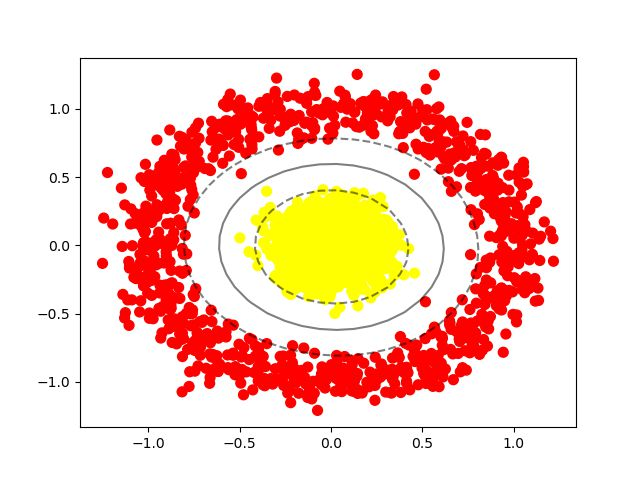
\includegraphics[width=0.4\textwidth]{images/0.jpg}

\end{center}


\begin{center}

 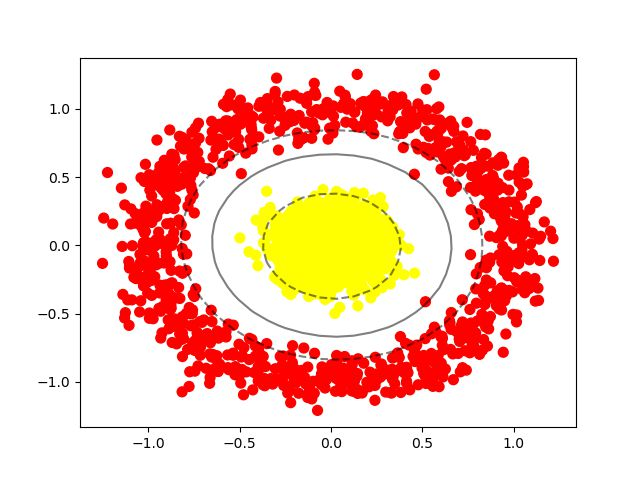
\includegraphics[width=0.4\textwidth]{images/1.jpg}

\end{center}


\begin{center}

 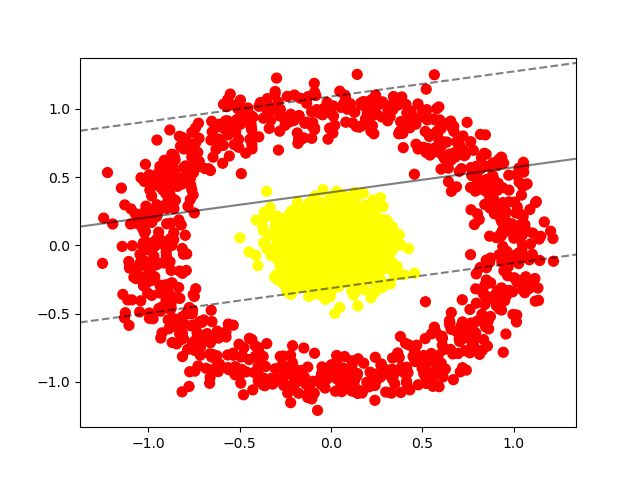
\includegraphics[width=0.4\textwidth]{images/2.jpg}

\end{center}

\begin{center}

 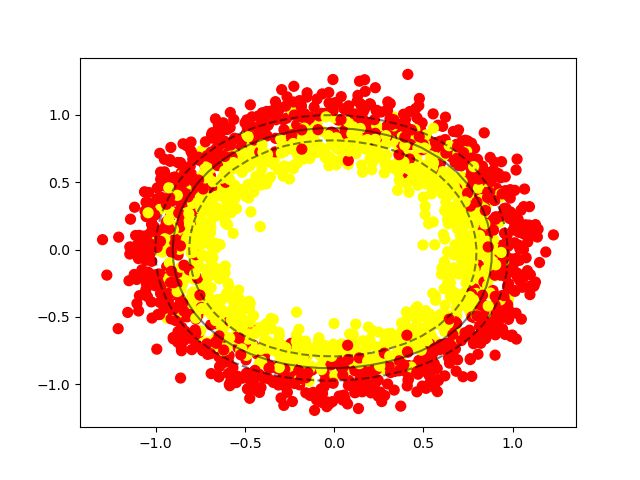
\includegraphics[width=0.4\textwidth]{images/10.jpg}

\end{center}


\begin{center}

 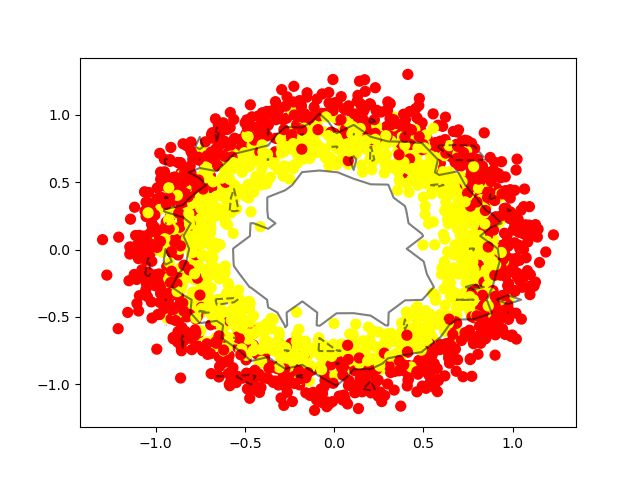
\includegraphics[width=0.4\textwidth]{images/11.jpg}

\end{center}


\begin{center}

 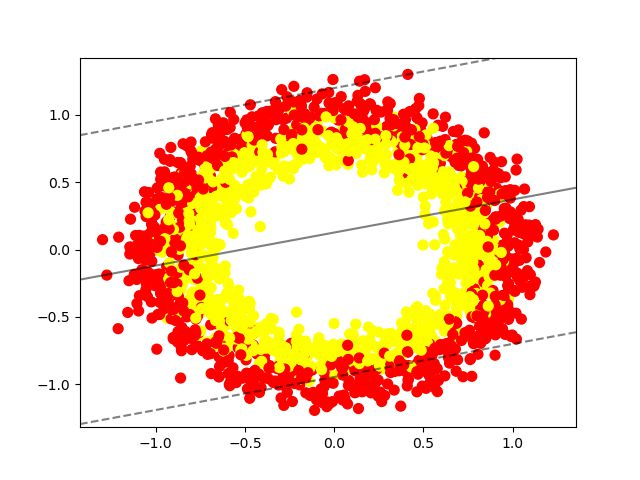
\includegraphics[width=0.4\textwidth]{images/12.jpg}

\end{center}

\begin{center}

 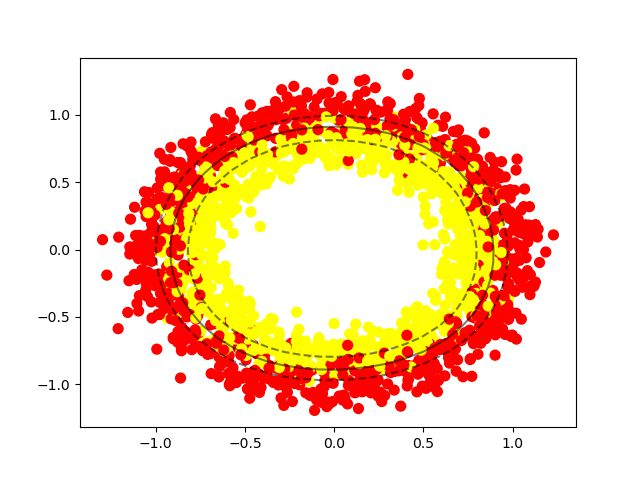
\includegraphics[width=0.4\textwidth]{images/13.jpg}

\end{center}


\begin{center}

 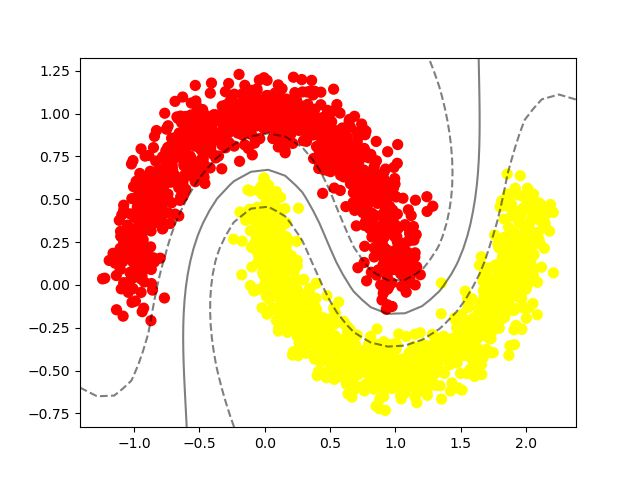
\includegraphics[width=0.4\textwidth]{images/20.jpg}

\end{center}


\begin{center}

 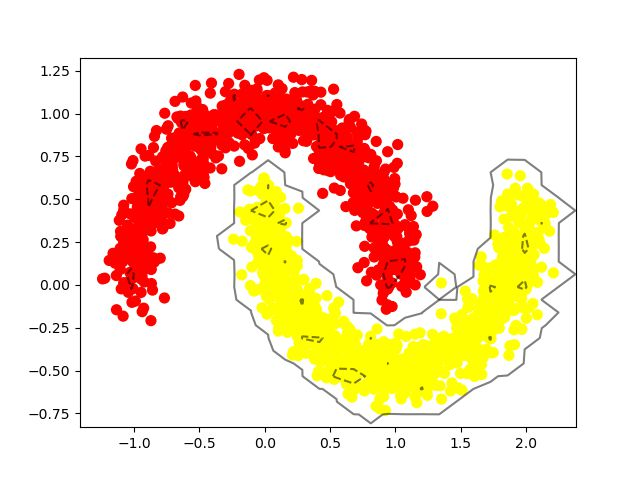
\includegraphics[width=0.4\textwidth]{images/21.jpg}

\end{center}


\begin{center}

 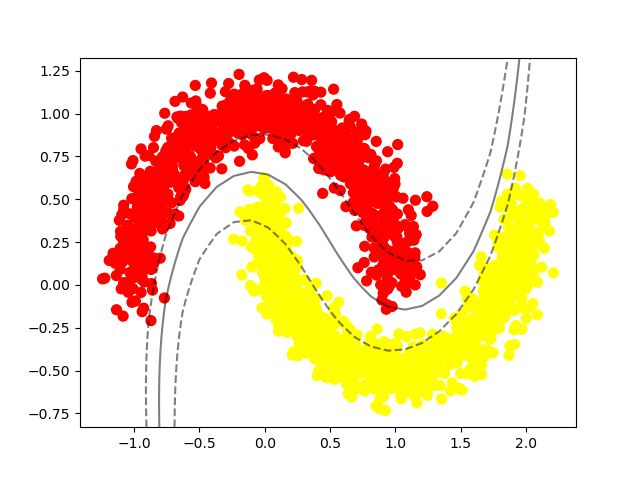
\includegraphics[width=0.4\textwidth]{images/22.jpg}

\end{center}

\begin{center}

 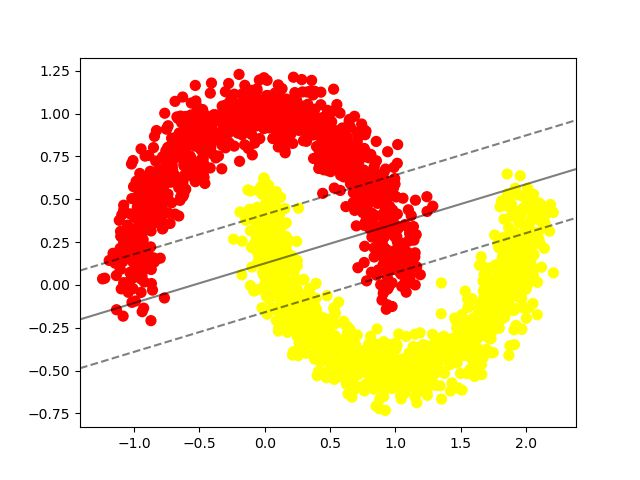
\includegraphics[width=0.4\textwidth]{images/23.jpg}

\end{center}

\begin{center}

 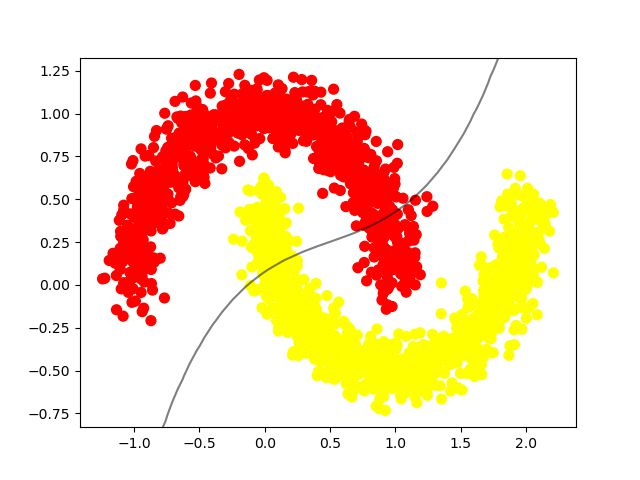
\includegraphics[width=0.4\textwidth]{images/24.jpg}

\end{center}


\begin{center}

 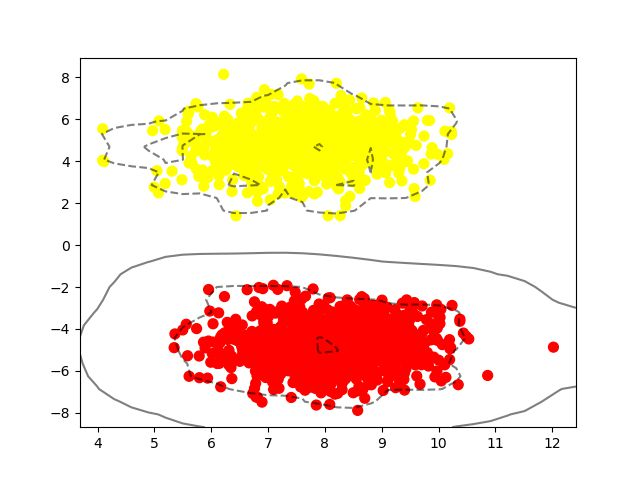
\includegraphics[width=0.4\textwidth]{images/30.jpg}

\end{center}


\begin{center}

 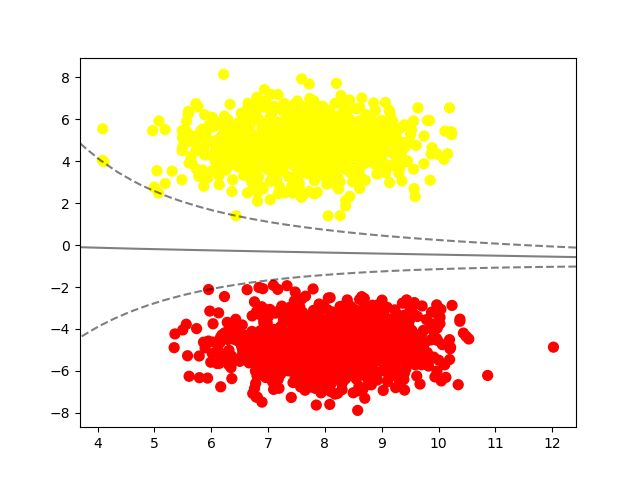
\includegraphics[width=0.4\textwidth]{images/31.jpg}

\end{center}


\begin{center}

 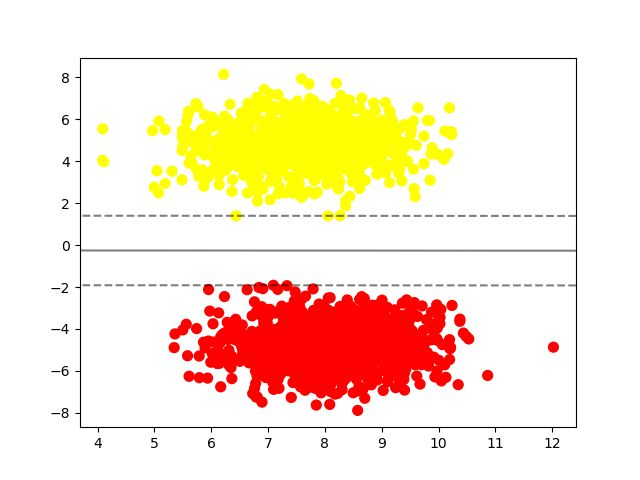
\includegraphics[width=0.4\textwidth]{images/32.jpg}

\end{center}


\begin{center}

 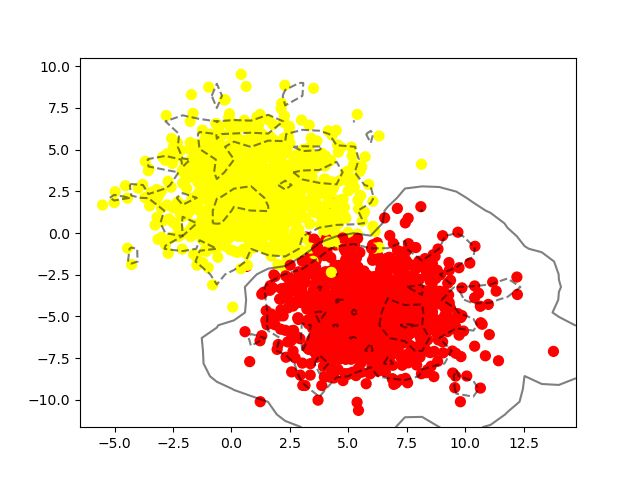
\includegraphics[width=0.4\textwidth]{images/40.jpg}

\end{center}

\begin{center}

 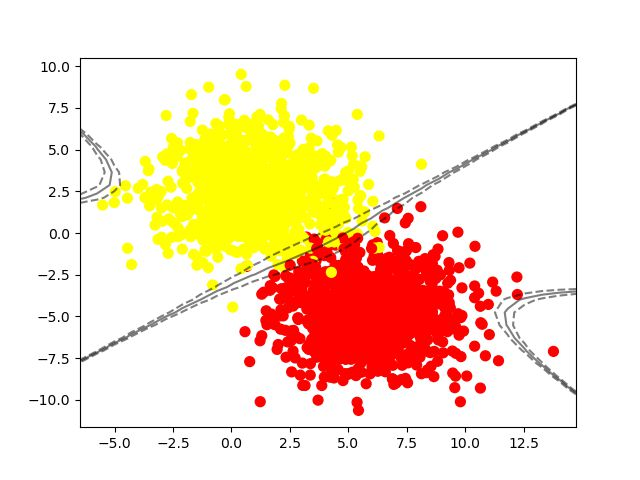
\includegraphics[width=0.4\textwidth]{images/41.jpg}

\end{center}

\begin{center}

 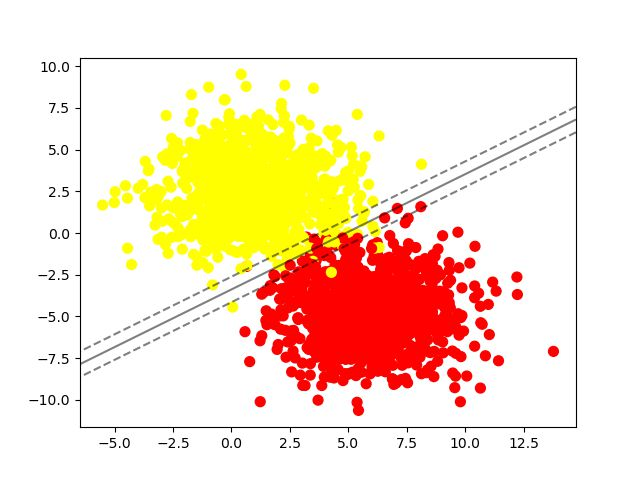
\includegraphics[width=0.4\textwidth]{images/42.jpg}

\end{center}

\newpage

\section{بخش دوم}

\subsection{توضیحات کد}

در پروژه شبکه عصبی، من از داده‌های MNIST که درون Keras قرار دارند و شامل 60000 تصویر اعداد دست‌نویس انگلیسی می‌شوند، استفاده کردم. در این جا هم از همین استفاده کردم.

در کدی که قرار داده‌ام، یک تابع \lr{kfold\_svm} وجود دارد که کاملاً مشابه بخش قبل است و بر اساس ورودی‌ها و کرنلی که به آن داده می‌شود، SVM را با \lr{Cross Validation} اجرا می‌کند. در ادامه برنامه این کدها برای لود کردن داده‌ها قرار داده شده است:



\begin{latin}
\begin{python}[language=Python]
MNIST_DS = keras.datasets.mnist
(train_images, train_labels), (test_images, test_labels) =
 MNIST_DS.load_data()

train_images = train_images / 255
test_images = test_images / 255


images = np.concatenate((train_images, test_images), axis=0)
labels = np.concatenate((train_labels, test_labels), axis=0)

number_of_samples = len(images)

images_flatten = images.reshape((number_of_samples,-1))
\end{python}

\end{latin}

و با این کد اجرا را انجام داده‌ام:


\begin{latin}
\begin{python}[language=Python]
clfs = []
scores = []
clf , score= kfold_svm(images_flatten[:],labels[:],
number_of_folds=2 ,kernel='linear' , C = 1)

clfs.append(clf)
scores.append(score)
print("best score" + str(scores))
\end{python}

\end{latin}


\subsection{نتایج}

چند نکته وجود دارد. من به طور کلی، چندین بار با کرنل‌های مختلف از جمله کرنل rbf و سایر کرنل‌ها بررسی‌هایی انجام دادم و در نهایت از نظر زمانی دیدم که کرنل خطی مناسب‌تر است. کرنل rbf هم در این جا نامناسب نبود ولی از نظر زمانی با توجه به ابعاد تصاویر، زمان زیادی طول می‌کشید. حال آن که در این جا چون عملاً در حالت خطی هم فضای ورودی‌ها $784$ بعدی است، همان کرنل خطی با زمان بهتری به نسبت rbf به جواب می‌رسد.

اما یک نکته وجود دارد و آن هم این است که SVM در اصل یک روش تئوری است که بدون هیچ نوع المان Random روی ورودی ثابت نتیجه یکسانی می‌دهد که در اثر تکرار اجرای یک الگوریتم به طور دقیق به دست آمده است و به نوعی نتیجه‌ای Deterministic دارد. نکته‌ای که این جا پیش می‌آید، این است که برای چنین فضای حالت بزرگی و به دلیل تعداد 60 هزار تایی داده‌های MNIST و این که کتابخانه sklearn از موازی سازی بهره نمی‌برد، عملاً اجرای الگوریتم زمان زیادی (در حد 20 دقیقه) نیاز دارد. البته اگر تعداد نمونه‌ها را در حد 1000 تا نگه داریم، زمان اجرا کاهش جدی پیدا می‌کند ولی الگوریتم svm در چنین حالتی به دلیل این که اندازه بعد ورودی تقریباً برابر تعداد داده‌ها می‌شود، به شدت دقیق می‌شود و به دقت $1$ و Overfit کامل می‌رسد و در نتیجه در تست به مشکل خواهد خورد و دقت 80 درصدی از خود نشان می‌دهد. از طرف دیگر در حالتی که با همه داده‌ها محاسبات انجام بشوند، در نهایت به دقت: $0.9792285714285714$ دست پیدا می‌کنیم.


به عنوان مقایسه‌ای با شبکه عصبی، همین مسئله دقت و زمان مطرح می‌شود. از نظر زمانی از آن جایی که sklearn موازی سازی نداشته و در این مورد خاص، تعداد داده‌ها هم برای SVM زیاد هستند و نیاز به محاسبات زیادی دارند، از نظر زمانی بسیار کندتر از شبکه عصبی می‌شود. در شبکه عصبی، کتابخانه tensorflow و Keras از موازی سازی هم روی CPU و هم در صورت در اختیار داشتن GPU های مناسب (مثلاً GPU های رده بالای شرکت NVidia) موازی سازی انجام گرفته و از سمت دیگر، از آن جایی که الگوریتمی تا حدی رندوم انجام می‌شود و همچنین در صورت استفاده از تعداد لایه‌های کم، محاسبات هم نسبت به SVM کمینه می‌شوند و به شکل بهینه‌تری هم انجام می‌شوند، شاهد بهبود زمانی فوق‌العاده هستیم. در حدی که هر Epoch از شبکه عصبی حدود 2 یا 3 ثانیه طول می‌کشد. از طرفی اما با SVM با صرف زمان زیاد، می‌توان به شکل قطعی و با آزمون و خطای کمتر، به دقت بسیار خوبی رسید و در تعداد نمونه کم، تقریباً به راحتی دقت 100 درصدی در SVM برای داده آموزشی مهیا شده و Overfit شدد رخ داده و نتیجه تست خوب نخواهد بود. در حالی که در شبکه عصبی دقت 100 درصدی در داده کم هم لزوماً مهیا نمی‌شود، اما سرعت عمل رسیدن به یک دقت معقول 97 تا 98 درصدی به شدت بهتر از SVM است.



\section{بخش سوم}
\subsection{توضیحات کد}

برای این قسمت ابتدا بعد از اکسترکت پوشه‌ها، یک کد در فایل \lr{file\_loader.py} نوشتم. وظیفه این کد این است که تمامی عکس‌های تمامی پوشه‌ها را در قالبی قابل فهم برای numpy از طریق matplotlib خوانده، در یک آرایه بزرگ numpy ذخیره کرده و همچنین در یک آرایه دیگر هم label ها را به همان ترتیب قرار بدهد و در نهایت کل فایل را به صورت npz که قابل باز شدن توسط numpy است ذخیره کند. در این قالب نام عکس ها با کلمه کلیدی images و نام label ها با کلمه کلیدی targets مشخص شده است و در نهایت یک فایل به نام \lr{persian\_lpr.npz} تولید می‌شود که از آن در کد اصلی برای لود کردن داده‌ها به کمک numpy استفاده می‌کنیم.

در فایل اصلی کد، همچنان هسته اصلی انجام SVM مشابه بخش‌های قبل است. برای آماده سازی کار از کدهای زیر استفاده شده است:


\begin{latin}
\begin{python}[language=Python]
dataset = np.load('persian_lpr.npz')
images = dataset['images']
labels = dataset['targets']

images = images/255
number_of_samples = len(images)
images_flatten = images.reshape((number_of_samples,-1))

\end{python}

\end{latin}

سپس با کدهای زیر با سه کرنل RBF با گاما 0.1، خطی و چندجمله‌ای درجه 6 با ضریب ثابت 1.2 عملیات دسته بندی انجام شده است و نتیجه داده تست بهترین Fold به همراه نتایج تست و یادگیری هر Fold تست  و یادگیری به نمایش در می‌آید.



\begin{latin}
\begin{python}[language=Python]
number_of_folds = 3

print("RBF:")
clf_rbf , score_rbf= kfold_svm(images_flatten,labels,
number_of_folds=number_of_folds ,kernel='rbf' , C = 1,gamma=0.1)
print("Best RBF accuracy= ",score_rbf)
print("--------------------")


print("Linear:")
clf_linear , score_linear= kfold_svm(images_flatten,labels,
number_of_folds=number_of_folds ,kernel='linear' , C = 1)
print("Best Linear accuracy= ",score_linear)
print("--------------------")

print("Poly Degree 6:")
clf_poly , score_poly= kfold_svm(images_flatten,labels,
number_of_folds=number_of_folds ,kernel='poly' ,
degree = 6 , coef0=1.2, C = 1)
print("Best Poly degree 6 accuracy= ",score_poly)
print("--------------------")

\end{python}

\end{latin}


سپس کد زیر هم قرار گرفته که از کاربر می‌پرسد آیا می‌خواهد نتیجه پیش بینی را برای یک عکس با Index خاصی که کاربر ورودی می‌دهد به همراه عکس مشاهده کند یا نه که در صورتی که یک وارد شود، Index از کاربر پرسیده شده و نتیجه پیش بینی هر کدام از SVM Classifier ها به همراه لیبل اصلی عکس و خود عکس به نمایش در می‌آید.


\begin{latin}
\begin{python}[language=Python]
do_test_images = input("Do you want to test an image?\n 1:Yes \t 0:No\n")
if (do_test_images=='1'):
    image_index = int(input("input image index: "))
    plt.imshow(images[image_index])
    plt.show()
    print("Images is: " ,labels[image_index])
    print('rbf predicts:'
     ,clf_rbf.predict([images_flatten[image_index]]))
    print('linear predicts:'
     ,clf_linear.predict([images_flatten[image_index]]))
    print('poly degree 6 predicts:' 
    ,clf_poly.predict([images_flatten[image_index]]))
\end{python}

\end{latin}


\subsection{نتایج}

به طور کلی، با هر سه کرنل گفته شده، توانستم نتایج خوبی به دست بیاورم. در اصل البته این موضوع با کمی تغییر دادن‌های مختلف در اعداد میسر شد تا در نهایت به حالت نسبتاً بهینه با مدت زمان اجرای بسیار کم و خوب برسم.

\begin{latin}
\begin{verbatim}
RBF:
train_scores: 
[0.977 0.979 0.976]

test_scores: 
[0.96  0.966 0.95 ]
Best RBF accuracy=  0.966
--------------------
Linear:
train_scores: 
[0.981 0.98  0.981]

test_scores: 
[0.956 0.968 0.962]
Best Linear accuracy=  0.968
--------------------
Poly Degree 6:
train_scores: 
[0.97  0.967 0.965]

test_scores: 
[0.954 0.966 0.964]
Best Poly degree 6 accuracy=  0.966


\end{verbatim}
\end{latin}

همان طور که از کد و نتایج بالا واضح است،  این نتایج در اثر اجرای \lr{Cross Validation} به صورت \lr{3-Fold} به دست آمده‌اند.


\newpage



\section{چالش‌ها}

از آن جایی که در بخش‌های قبل نتایج هر بخش را هم شرح دادم، بخش انتهایی را به چالش‌هایی که با آن رو به رو شدم اختصاص داده‌ام.


چالش اولیه کار، یادگرفتن کار با توابع SVM کتابخانه sklearn بود که خوشبختانه پیچیدگی خاصی نداشتند و به راحتی انجام شدند. چالش بعدی پیدا کردن توابعی بود که داده‌های مورد نیاز ما را به شکل اتوماتیک تولید نمایند. برای این کار با جست و جو در اینترنت، به توابع آماده \lr{make\_blobs} و \lr{make\_circles} و \lr{make\_moons} که در sklearn قرار دارند، رسیدم که برای این تمرین مناسب بودند و از آن‌ها استفاده کردم.

چالش بعدی پروژه برای بخش دوم آن و مشکل زمان بود که در ابتدا برای توابع RBF تست می‌کردم و به دلیل سربار محاسباتی بیش‌تر، زمان آن خیلی زیاد می‌شد، اما در نهایت با بررسی حالت \lr{2-Fold} جداکننده خطی، دیدم که می‌توان به نتایج خوبی دست یافت و در نتیجه، از همان استفاده کردم.

در نهایت برای بخش آخر چالش اصلی این بود که کاری کنم که داده‌های قرار داده شده به صورت عکس، به شکل منظوم و ساماندهی شده و قابل لود کردن به صورت یک جا در بیایند که با کمک فرمت npz و savez در numpy این امر به خوبی محقق شد.



\end{document}













